\chapter{Background and Related Work}
\label{chapter:background}

\section{Fire Models}
\subsection{Overview}
In order to build a forest fire simulator, forest specific data must be integrated. Rothermel developed the first eleven fuel models that are still used to this day \cite{roth}. The method by which these eleven fuel models were created is the basis for the development of all modern fuel models. The fuel model contains information on properties of the forest in a particular region, and at a certain granularity. The forest is broken up into cells, each cell having properties which are modeled in the fuel model. For example, one fuel model might describe a coniferous forest in regions of 30x30 meter cells. These cells are what make up the basis for a fire simulation. 
 

\subsection{Fire Shape}

The majority of the existing forest fire simulators, including this work, calculate wildfire spread based on the Rothermel's fire spread equations \cite{roth}. More detail on the simulators which use this fire spread model will be covered later in the section. Equation \ref{eq:roth} shows his rate of spread equation, which is based on several parameters. 

% \begin{equation}\sum_{i=0}^{\infty}x_i=\int_{0}^{\pi+2} f\end{equation}
\begin{equation}
R = \frac{(I_{p})_{o}(1 + \phi_{w} + \phi_{s})}{\rho_{b}\varepsilon Q_{ig}}
\label{eq:roth}
\end{equation}

Where R is the rate of spread, $(I_p)_o$ is the no-wind propagating flux, $\phi_w$ and $\phi_s$ are the additional propagating flux introduced by wind and slope respectively. The product of $\rho_b$ and $\varepsilon$ is referred to as the effective bulk density. The effective bulk density models the amount of fuel per unit volume of the fuel bed raised to ignition ahead of the advancing fire. $Q_ig$ is the heat of preignition (the heat required to bring a unit weight of fuel to ignition). These values are derived or contained in the fuel model that describes the cell for which the computations are being done. 

The desired output from a forest fire simulator is a time of arrival map. Each cell in this time of arrival map represents a cell in the simulation forest, and the value it contains is the time at which the cell ignited and started propagating the fire. Once a cell is lit, it begins contributing to the spread of the fire to the surrounding cells and continues burning until the fuel in that cell is entirely used. The method of propagation may vary between simulators, but the basic spread rate is usually based on Rothermel's equations.

%\subsection{Model Subsystems}

\subsubsection{Surface Fire}
There are several potential approaches to calculating the propagation of the fire. This paper implemented three methods for iterating through a simulation to calculate the time of arrival map for a simple one-source forest fire under constant terrain and wind conditions. The first two spread methods (Minimal Time and Iterative Minimal Time) are based on stepping through time independent of specific fuel conditions and are based on the paper by Sousa, dos Reis, and Pereira \cite{gpufire}. The third spread method implemented in this paper (Burn Distances) was based on code and methods found in vFire \cite{vFire}. vFire implemented an accurate spread rate calculator based on Rothermel's fire spread equations and the fire spread and fuel model data to propagate based upon the physical burning of fuel.

Sousa et. al. also used the GPU to improve their running times and ported fireLib to the GPU \cite{gpufire}, but were the first to use the parallel programming language CUDA \cite{cuda}. They implemented three kernels in which they explored three different propagation types. This paper based two of the spread methods (Minimal Time and Iterative Minimal Time) on the work done by Sousa, dos Reis, and Pereira. 

\begin{figure}%[!t]
\centering
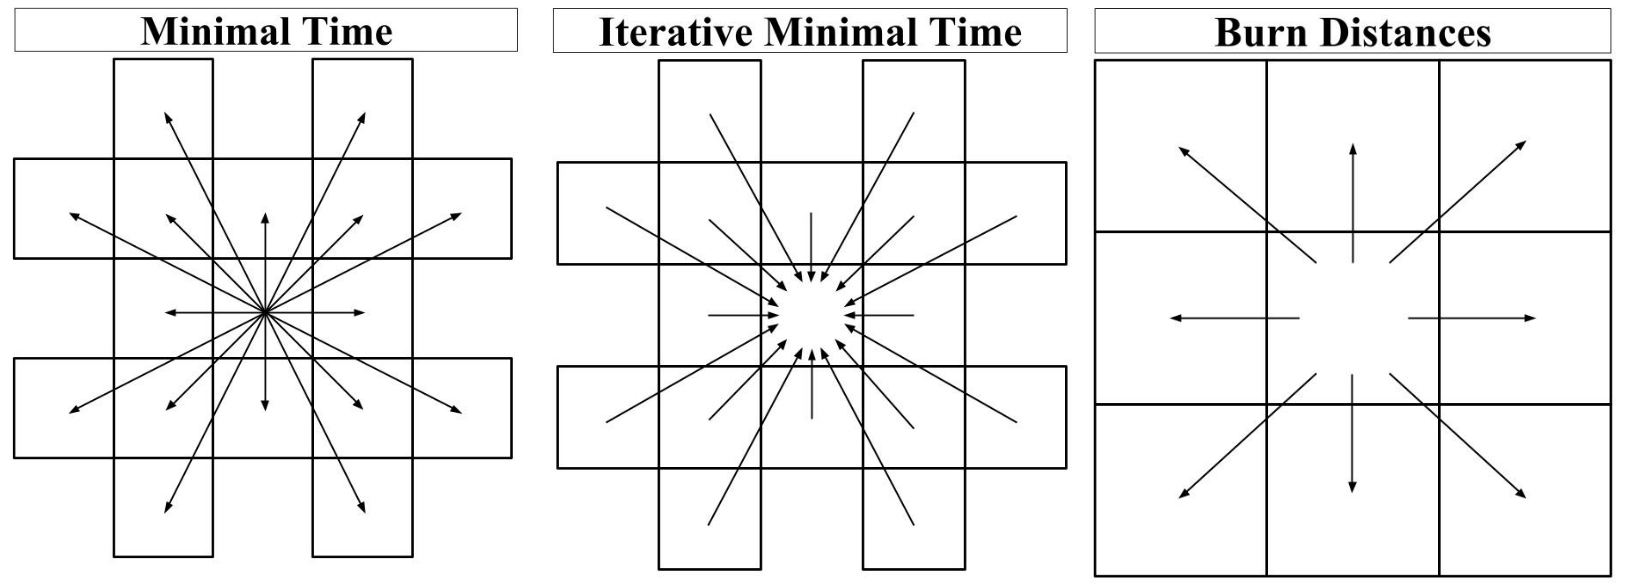
\includegraphics[width=\linewidth]{figures/background/spread_methods.PNG}
\caption{Neighbor access methodology for each of the propagation methods. From left to right: Minimal Time, Iterative Minimal Time, Burn Distances}
\label{fig:spreadTypes}
\end{figure}

\paragraph{Burn Distances}
The Burn Distances (BD) method is based on the idea that it takes a certain amount of time for fire to burn the distance between two cells. This distance is set as equivalent between all cells and these properties are computed and loaded in the preprocessing stage of the program. Since they are handled in preprocessing, they are based on the properties of the forest model which is based on the size of the forest cell. The simulation iterates at a constant time step, and the amount the distance has burned is tracked throughout all the time steps. 

\paragraph{Minimal Time}
The Minimal Time (MT) propagation method uses a dynamic time stepping method to step through the simulation. At each time step, a cell is examined to see if it is on fire. If the cell is burning, then the neighbors of the cell are examined as seen in Figure \ref{fig:spreadTypes}. If the neighbor is already on fire, it is ignored. If the neighbor is unlit, then the time of arrival for that cell is computed using the propagation equation found in Equation \ref{eq:rate}. In the Minimal Time method, time is incremented dynamically. Each time a new ignition happens, the ignition time is compared to the current 'timeNext' variable. If the new ignition time is smaller (the fire arrives sooner) than the current timeNext, then it replaces the timeNext value. This methodology means that time is incremented based on which cell will ignite the earliest.

\paragraph{Iterative Minimal Time}
The Iterative Minimal Time (IMT) method is designed to avoid data dependencies. Each cell operates independent of its neighbors, calculating the ignition time based on the spread rates, and only finishing when the values between step $k$ and $k + 1$ converge. Each cell looks at the minimal time for each of its neighboring cells to burn towards it as shown in Figure \ref{fig:spreadTypes}. The value is known to converge after the difference between two time steps is less than some small threshold. The most appropriate value for this threshold can be determined through experimentation.

\subsubsection{Crowning}
Crowning is the phenomena of the fire moving from spreading along the base of the forest to up the trees to their crowns. There are two types of crowning: passive and active. A passive crown fire is one which does not spread to the overall propagation of the fire. Conversely, an active crown fire does contribute to the spread of the fire. CITATION.

\subsubsection{Spotting}
Spotting occurs when fire brands from the wildfire are lifted into the air and fly ahead of the flame wall to start small fires ahead of the advancing fire wall. This incident occurs when Torching occurs. Torching occurs when the fire spreads from the base of the forest to the tree-tops. It does not contribute to the spread of the fire. CITATION? AND (other times spotting occurs)? 

\section{Fire Simulators}
Since Rothermel's paper was published in 1972, several fire spread simulators have been developed. Every major forest fire simulator has used his spread equations as the basis for their simulation. The first major fire spread simulator was developed in 1986 called BEHAVE\cite{BEHAVE}. BEHAVE had two main functions to the application. The first function allowed users to load in fuel models from Rothermel's paper, but also to develop and save new fuel models. The simulator then had the ability to integrate the newly developed fuel models in its simulations. The second function of the application would run a simulation and burn prediction on the desired fuel model. The output of this simulator appeared in a table which represented the times of arrival for each cell in the simulation. There was no visualization method available for this simulator. The simulation was meant to be used as a training tool rather than a real-time tool to be used to fight wildfires. 

\subsubsection{fireLib}
A decade later in 1996, BEHAVE was the basis for a new forest fire library that was developed using C called fireLib \cite{fireLib}. The code was based entirely on BEHAVE's simulator, but brought up to a then-modern platform. FireLib can run much faster than BEHAVE, and the output is given in time of arrival arrays rather than a table. Each (x,y) in the array corresponds to a cell in the fire simulation, and the time of arrival is the time at which the cell ignites, and can then begin to propagate the fire. The fire library is more flexible than BEHAVE and allows a user to design their own methods for propagating the fire. There are a few different methods which may be used, and will be addressed later in the paper. However, where BEHAVE was an entire application which had an interface component, fireLib is simply an open source forest fire library and both the visualization and interface development are left up to the user.

\subsubsection{FARSITE}
In 2004, FARSITE was developed, which works as a full-scale forest fire simulator \cite{FARSITE}. It has been continuously developed since 2004 and is currently still operational. It incorporates more features than simple fire spread, such as crown fires, surface fires, fire acceleration, and spotting. While it is one of the most advanced and accurate forest fire simulators, it is not very fast. It is one of the most widely used forest fire simulators in existence today.

\subsubsection{vFire}
This paper used much of the fire spread implemenation from a forest fire simulator called vFire \cite{vFire}. vFire was based on hFire, and are both cellular based spread models. They run faster than FARSITE, but do not have the same level of precision \cite{hFire}. vFire uses a technique that has dynamic time stepping to burn distances between cells to determine an accurate time of arrival for the fire spread. The important feature that vFire accomplished was porting the computation of the fire spread to the GPU using OpenGL shaders \cite{opengl}. Because the computation was ported to the GPU, it accomplished a very high speedup over its sequential implementation. 

\section{GPU Computation}
\subsection{Overview}
% History from CUDA site:
% http://www.nvidia.com/object/cuda_home_new.html
GPU's were originally designed as graphics accelerators supporting only very specific fixed-function pipelines. This meant that using them for high performance computation was not easy unless it could be integrated with some sort of visualization language. An example of such an integration may be seen in vFire \cite{vFire}. In 2006, NVIDIA released CUDA, which was the world's first solution to general-purpose computing on the GPU. Ever since its release, and even beforehand, the GPU was used for its high-processing capabilities. The architecture of the GPU allows for hundreds of low-powered processors to run in parallel. This type of computation is ideal for situations where the same computation to hundreds of inputs. The pitfalls of GPU computation occur when data dependencies exist in the data. If one portion of the data must wait on another to finish, it limits the usefulness of the GPU for processing. 

\subsection{CUDA}
CUDA (Do I need the little (R) symbol?) is a parallel computing platform and computing model created by NVIDIA. It harnesses the hundreds of cores provided by a GPU an allows programmable kernels to be written. A GPU can allocate blocks and threads. Blocks are XX. Threads are XX. 

** Mention CUBIX here

\section{Data}
Here is where I want to put a section on the fuel/moisture/etc models. Roger didn't include anything about this and it would have been helpful. But first I must figure out what to write. 

\subsection{Fuel Models}
\subsection{Moisture Models}